	%%%%%%%%%%%%%%%%%%%%%%%%%%%%%%%%%
%% Ersetzen Sie in den folgenden Zeilen die entsprechenden -Texte-
%% mit den richtigen Werten.
\documentclass[course=erap]{aspdoc}
\newcommand{\theGroup}{167} % Beispiel: 42
\newcommand{\theNumber}{A212} % Beispiel: A123
\author{Nicolas Arteaga \and Manuel Cardenas \and Erick Quintanar}
\date{Sommersemester 2019} % Beispiel: Wintersemester 2018/19
%%%%%%%%%%%

% Diese Zeile bitte -nicht- aendern.
\title{Gruppe \theGroup{} -- Abgabe zu Aufgabe \theNumber}

\begin{document}
\maketitle

\tableofcontents

\section{Einleitung}\label{section:einleitung}

Diese Dokumentation wurde im Rahmen des Rechnerarchitektur-Praktikums im Sommersemester 2019
angefertigt. Das Praktikum Rechnerarchitektur ist eine Veranstaltung des Lehrstuhls für Rechnerarchitektur und Parallele Systeme an der Technischen Universität München, welche im Zuge des Informatik B.Sc. Studiums absolviert wird. Unsere Aufgabe war es, einen Multicorn Fractal mittels Assembler erstmal zu berechnen und dann in einem Bild darzustellen. \\

Diese Ausarbeitung ist in 7 Teile unterteilt. Die \hyperref[section:einleitung]{\textbf{Einleitung}}, wo Sie sich jetzt befinden, soll einen kleinen und pr\"agnanten \"Uberblick des Praktikums darstellen. In die \hyperref[section:problemstellung]{\textbf{Problemstellung und Spezifikation}} wird die Aufgabenstellung, die einen Interpretätionsspielraum l\"asst, n\"aher analysiert und spezifiziert. Die \hyperref[section:losungsfindung]{\textbf{L\"osungsfindung}} erkl\"art wie wir die davor vorgestellte Aufgabe gel\"ost haben und unsere \"Uberlegungen dahinter werden auch ausf\"uhrlich erkl\"art. Die \hyperref[section:dokumentation]{\textbf{Dokumentation der Implementierung}} erk\"art wie unsere Implementierung funktioniert und im Kapitel \hyperref[section:ergebnsse]{\textbf{Ergebnisse}} wird das Resultat genau beschrieben. Als aller letztes geben wir eine kurze \hyperref[section:zusammenfassung]{\textbf{Zusammenfassung}} des ganzen wieder. \\

Falls Sie auf noch weitere Unregelmäßigkeiten treffen oder einen Fehler gefunden haben, melden Sie sich bitte bei uns unter einer der folgenden E-Mail-Adressen: \\
erick.quintanar@hotmail.com, nicolas.arteaga@tum.de, cardenam@in.tum.de

\section{Problemstellung und Spezifikation}\label{section:problemstellung}

\subsection{\"Uberblick}
In unserer Projektaufgabe mussten wir theoretisches Wissen aus der Mathematik anwenden, um einen Algorithmus in Assembler zu Implementieren, der eine bestimmte Art von Multicorn-Fraktal darstellen soll: der Tricorn-Fraktal. Im folgenden erkl\"aren wir unsere \"Uberlegungen zu der offenen Projektaufgabe und was f\"ur Annahmen wir bei der Ausarbeitung treffen mussten. 

\subsection{Theoretischen Teil}

Der Multicorn Fractal ist durch folgende Formel beschrieben:

\begin{equation}\label{eq:multicorn}
    z_{i+1} = \overline{z_i}^m + c \; (i > 0)
\end{equation}

Wobei $z_i$ innerhalb der complexen Ebene zu betrachten ist. Da wir einen Tricorn-Fractal implementieren sollten, gilt im folgendem:

\begin{equation}\label{eq:tricorn}
    z_{i+1} = \overline{z_i}^2 + c \; (i > 0)
\end{equation}

Man f\"angt dabei mit $z_0 = 0$ an und $c$ wird aus den Koordinaten der Komplexen Ebene gew\"ahlt. Das hei{\ss}t, man variiert $a$ und $b$ in $c = (a + bi)$ f\"ur $a \in [a_1;a_2]$ und $b \in [b_1;b_2]$, wodurch verschiedene $z_n$ f\"ur jedes eingesetzte $c$ entstehen. Weiter unten, im \hyperref[problemstellung:praktisch]{praktischen Teil} der Aufgabenstellung wird die Wahl von $a_1, a_2, b_1$ und $b_2$ genauer erkl\"art. 

\begin{itemize}
    \item Aus \eqref{eq:tricorn} berechnen wir Real- sowie Imagin\"arteil in $z_{i+1}$ f\"ur jedes m\"ogliche $c$ innerhalb unserer durch $a_1, a_2, b_1$ und $b_2$ beschr\"ankten Intervalle.  
    \item Aus dem Ergebnis von $z_i$ kann man herausfinden, ob f\"ur das gegebene $c$ die Formel beschr\"ankt ist. Dadurch kann man das Pixel, der zu $c$ korrespondiert entweder schwarz oder f\"arbig (Die gew\"ahlte Farbe beschreibt, wie unbeschr\"ankt das eingesetzte $c$ ist, d.h. wie viele Iterationen gebraucht werden, um zu merken, dass $z_i$ tats\"achlich unbeschr\"ankt ist) darstellen. 
    \item Die Formel l\"asst sich durch benutzung von SIMD f\"ur vier verschiedene Werte von $c$ gleichzeitig berechnen. 
\end{itemize}

\subsection{Praktischen Teil}\label{problemstellung:praktisch}

In der Datei mit dem Assemblercode mussten wir die Function \\

\lstinline{void multicorn(float r_start, float r_end, float i_start, float i_end, float res, unsigned char* img)} \\

implementieren, welche die Ergebnisse f\"ur alle $c = a + bi$ im Bereich $[a_1, a_2]$ und $[b_1, b_2]$ mit $a_1 = $ \lstinline{r_start}, $a_2 = $ \lstinline{r_end}, $b_1 = $ \lstinline{i_start} und $b_2 = $ \lstinline{i_end} berechnen sollte. Das Attribut \lstinline{res} soll dabei die Resolution des Bildes sein und das Attribut \lstinline{img} ein Pointer auf die Adresse zur Bitmap datei, wo die Tricorn Menge gezeichnet werden soll. \\

Dazu muss man f\"ur jedes $z_i$ bestimmen, ob die Formel nach einem beliebigen aber fixen $i$ (Anzahl Iterationen) beschr\"ankt ist oder nicht, und dazu das zugeh\"orige bit schwarz malen. Wenn es nicht beschr\"ankt ist, muss der dazu geh\"orige Pixel farbig gemalt werden. Es muss auch gelten, dass der reelle- sowie auch der imagin\"are Bereich, gegeben durch den Benutzer mit \lstinline{r_start, r_end, i_start, i_end}, eingehalten wird. Die Resolution des Bildes, d.h. wie scharf es aussehen soll, wird vom Benutzer durch das Attribut \lstinline{res} gegeben. Das letzte Attribut \lstinline{img} soll ein Pointer zum Speicherplatz einer 24-bit BMP Datei sein, dieser muss aber nicht vom Benutzer kommen, sondern anderseits von einer in C geschriebenen Datei, die alle I/O Operationen behandeln muss. \\ 

\subsection{Fazit}

\textbf{TODO: Fazit ähnlich zu Zussamenfassung, kleiner machen bzw. Dinge in zsf. schreiben}

Zussammengefasst haben wir also eine Aufgabe bekommen, wo wir mittels Assembler einen Tricorn Fractal abh\"angig von verschiedenen Eingaben des Benutzers berechnen sollen. Nach den ganzen Berechnungen muss also eine Datei wie oben in der Abbildung zu sehen \ref{fig:tricorn_expected}, entstehen. Diese darf aber auch gef\"arbt werden, da die verschiedenen Farben beschreiben, wie unbeschr\"ankt das aktuelle Pixel (also wie unbeschr\"ankt das $z_i$ mit verschiedene $c$ Koordinaten) ist. 

\begin{figure}
    \centering
    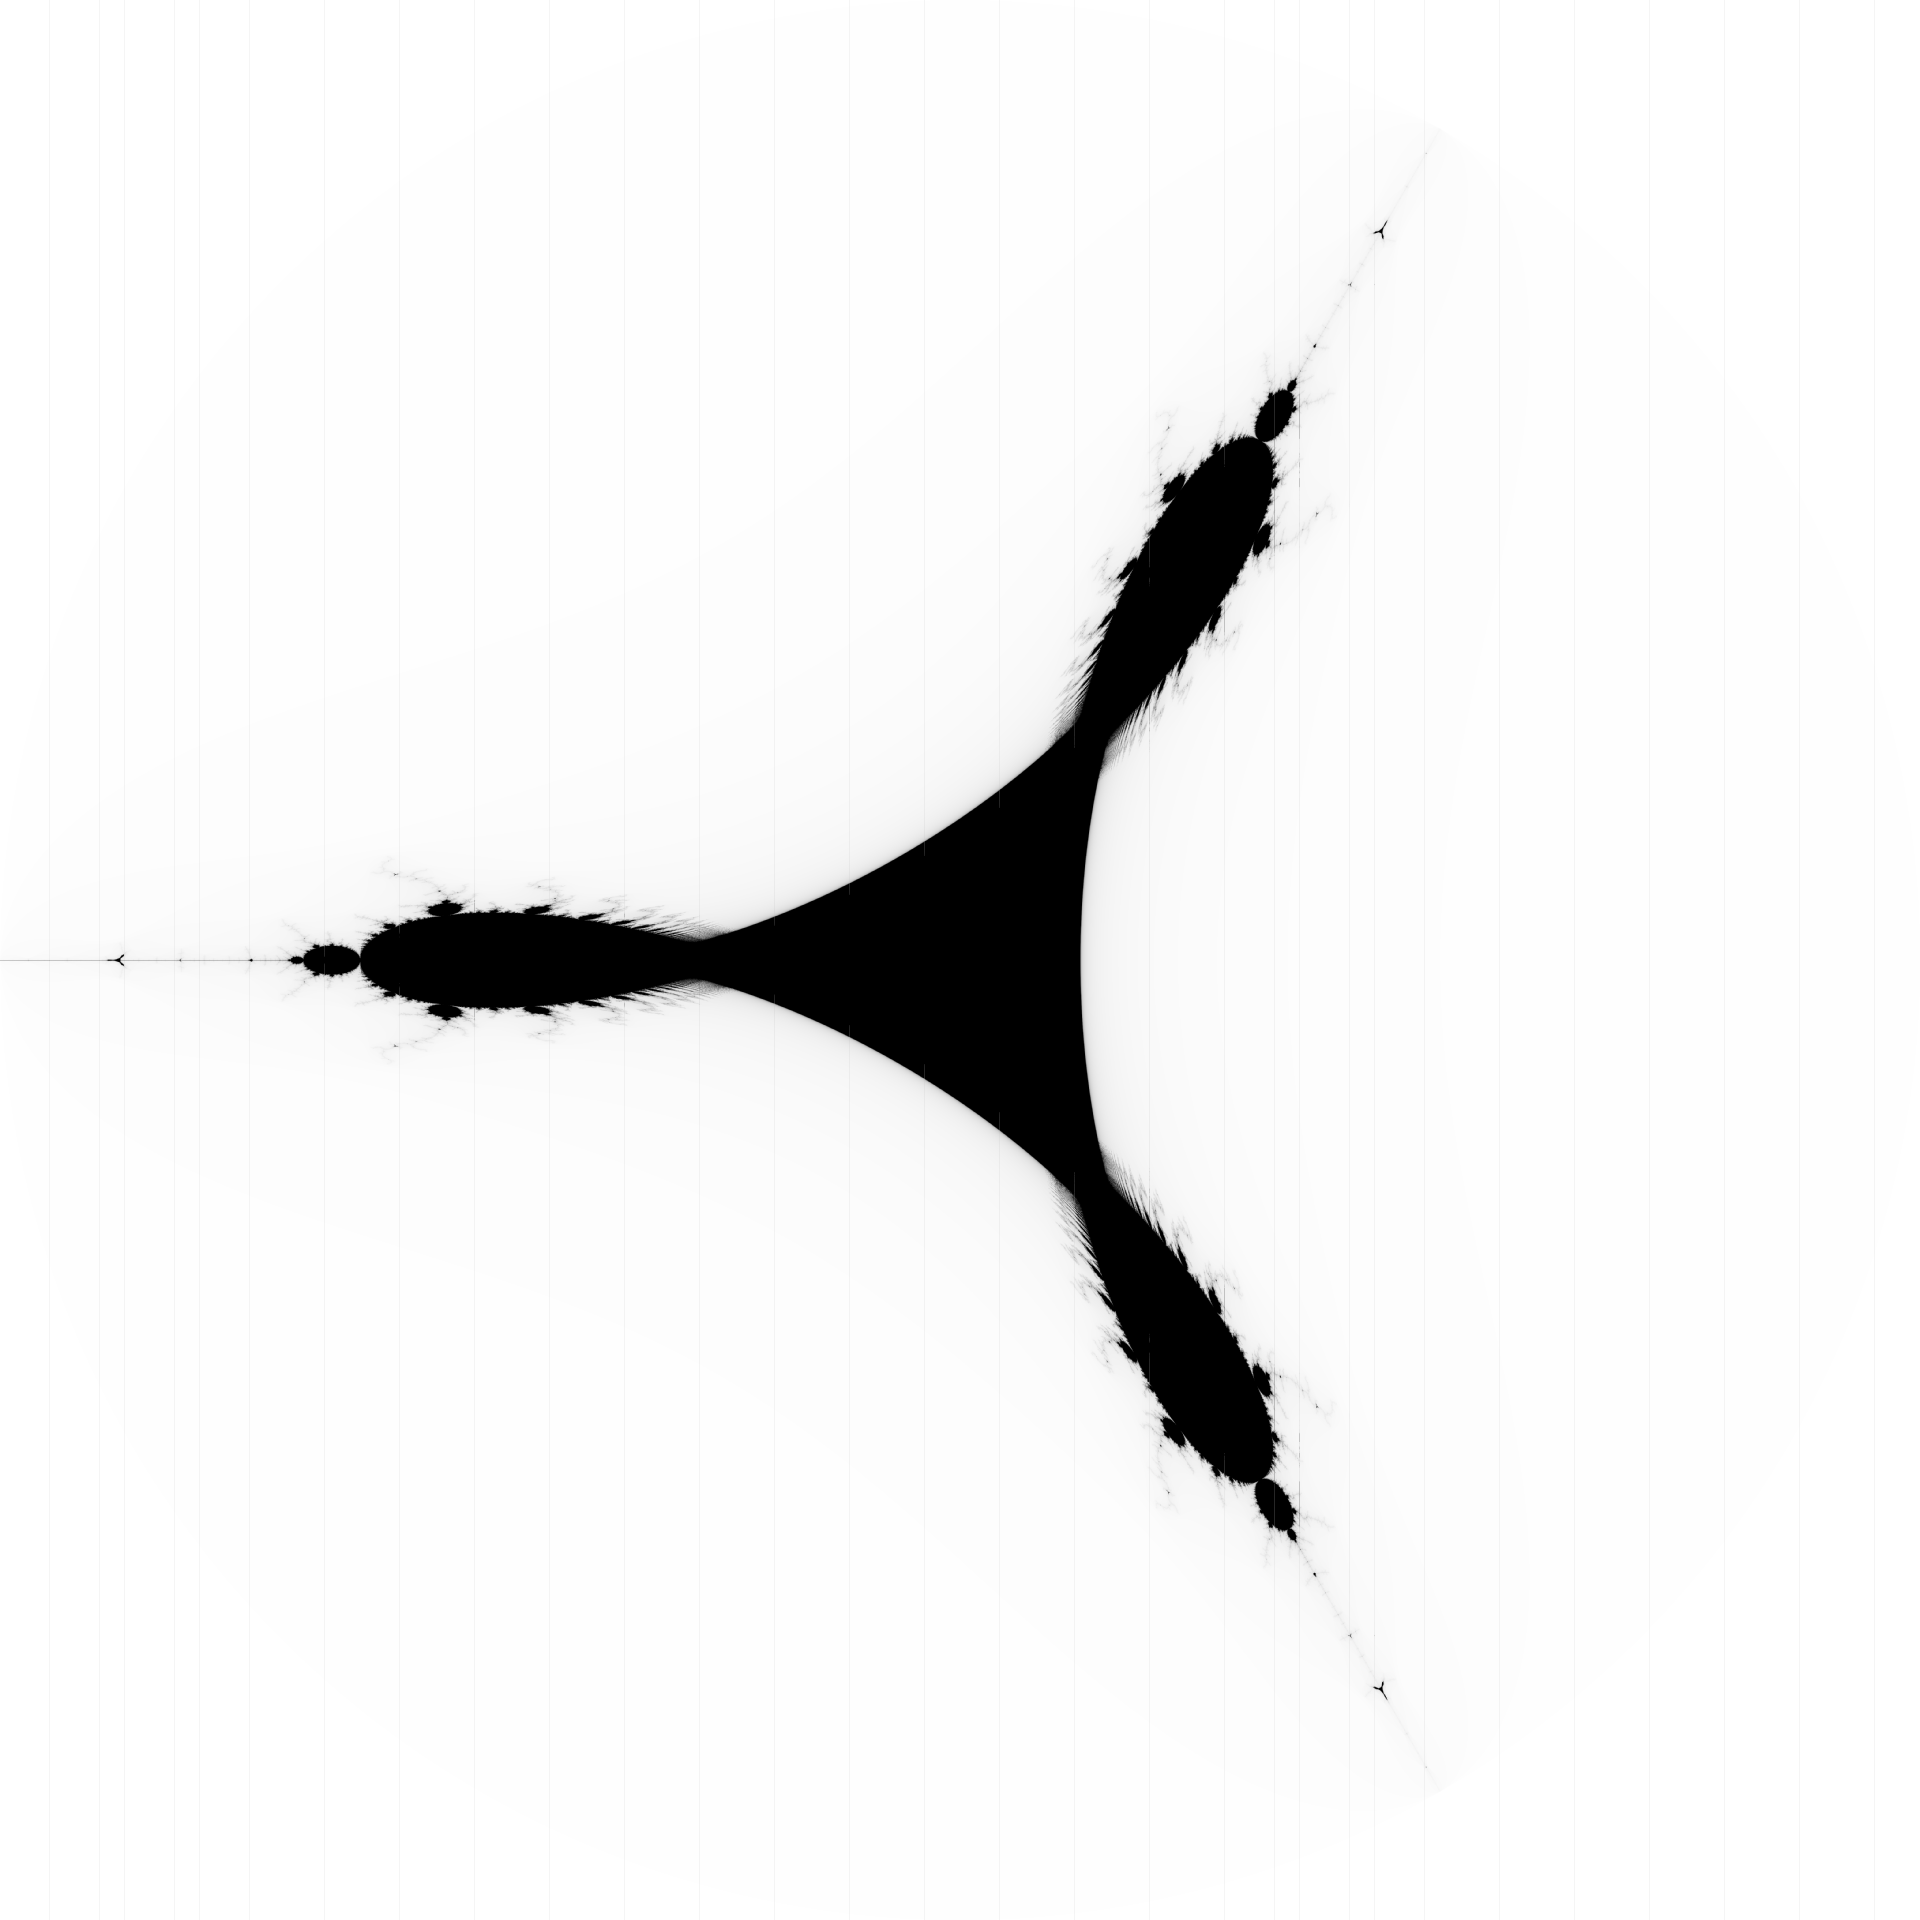
\includegraphics[width=100mm]{img/Tricorn_expected.png}
    \caption{Wie einen Tricorn Fractal laut Wikipedia aussehen soll \cite{tricorn_expected}}
    \label{fig:tricorn_expected}
\end{figure}

\section{Lösungsfindung}\label{section:losungsfindung}

Mit einem klaren Verst\"andnis der Aufgabe, sind wir nun zur Implementierung gesprungen. Im folgenden Kapitel erkl\"aren wir unseren Weg zur L\"osung. Dazu z\"ahlt, welche Fragen entstanden sind und wie wir diese gel\"ost haben, welche Probleme w\"ahrend der Implementierung entstanden und wie wir diese behoben haben. Also im Allgemeinen erkl\"aren die n\"achsten Abs\"atze unsere Entscheidungen und wie diese zu eine Funktionalen Implementierung gef\"uhrt haben. 

\subsection{Erste Fragen}

Nach genauerem Anschauen der Funktion, die wir in Assembler implementieren sollten: \\

\lstinline{void multicorn(float r_start, float r_end, float i_start, float i_end, float res, unsigned char* img)} \\

entstanden erstmal einige Fragen. Zuerst haben wir uns überlegt, wie wir das Attribut \lstinline{res} betrachten sollten. Die Resolution kann auf zwei verschiedene Weisen interpretiert werden. Entweder als die Grö{\ss}e von jedem Pixel, zum Beispiel, wenn res $0.1$ ist, dann wäre die Höhe des Bildes 20 Pixel lang und die Breite 30 Pixel, da zwanzig $0.1$ Schritte gemacht werden m\"ussen um von -1 zu 1 zu laufen. Bei unserer Implementierung haben wir \lstinline{res} als ein Skalar des Bildes betrachtet, der die Breite und Länge multipliziert. Also, 100 mal unsere Resolution 3x2  wäre am Ende 300x200 Pixel. Das hei{\ss}t, dass wir aus dem eingesetzten \lstinline{res} auch die entsprechende Skalierung von jedem Pixel durch $1/res$ berechnen k\"onnen. \\

Die Zweite Frage die wir beantworten mussten, ist wie die Berechnung \"uber die Beschr\"ankung von $z_i$ sein soll. Dazu haben wir uns erstmal entschieden, dass, wenn nach $i$ Iterationen der Wert von $z_i$ aus dem reellen Bereich $[-2, 1]$ oder aus dem Imagin\"aren Bereich $[1, -1]$ herausrutschen sollte, es als unbeschr\"ankt gelten soll und dadurch der Pixel der dem Entsprechenden $z_i$ entspricht (d.h. der Pixel der dem gegebenen $c$ entspricht) musste als Unbeschr\"ankt dargestellt werden. Nach einigem Ausprobieren haben wir gemerkt, dass der Bereich $[-2, 2]$ f\"ur Imagin\"are und Reelle Werte bessere Ergebnisse hervorbringt. \\

Auf der Anderen Seite ist ein $z_i$ beschr\"ankt, wenn es nach einer Fixen Anzahl $R$ von $i$ Iterationen, nicht nach obiger Definition unbescr\"ankt ist. Wir haben $R$ durch einfaches Ausprobieren zu $R = 100$ gesetzt. Es hat sich herausgestellt, dass $R = 50$ die Sch\"arfe des Bildes verringert und dass der Unterschied zwischen $R = 200$ und $R = 100$ zu niedrig war, damit sich die weiteren Iterationen lohnen.

\subsection{Technische Entscheidungen}

\subsubsection{Eingabe}

In Bezug auf die Eingabe des Codes gibt, wie oben erkl\"art, die Projektaufgabe an, dass der Benutzer in der Lage sein soll, die Aufl\"osung des Bildes, sowie die Bereiche komplexer Zahlen, getrennt in Real- und Imagin\"arteile, zu senden. Diese Eingaben werden dann zur Durchf\"uhrung der Berechnungen verwendet. Aus diesem Grund haben wir die Auswirkungen der Eingabedaten auf die Berechnungen ausf\"uhrlich \"uberlegt, damit wir auch Sicherheitsmethoden implementieren k\"onnen, um unkorrektes Codeverhalten zu vermeiden. \\

Wir stellen fest, dass die Aufl\"osung nicht Null sein kann, da keine definierte Berechnung stattfinden w\"urde (wir teilen ja eins durch \lstinline{res}), und dass die Aufl\"osung nicht gr\"oßer als 5000 sein kann, da die Datei, in der sich das Ergebnis befindet, viel zu viel Speicherplatz (ca. 500 MB) belegen w\"urde. Wir haben uns auch daf\"ur entschieden, dass die Bereiche der imagin\"aren Zahlen sowie der reellen Zahlen nicht Null sein d\"urfen und dass der Anfang des Bereichs immer kleiner als das Ende sein sollte, da das Programm in beiden F\"allen nichts berechnen wu\"urde. Schließlich \"uberpr\"uft der Code, ob der Benutzer alle erforderlichen Argumente geschrieben hat, um die Berechnung ohne Fehler durchf\"uhren zu k\"onnen. \\

Es sollte auch beachtet werden, dass die Argumente, die der Benutzer in der Konsole schreibt, als Argumente \"ubergeben werden und dass diese von Strings in Floats umwandelt werden m\"ussen, damit sie sp\"ater bei der Berechnung des Fraktals verwendet werden k\"onnen. Auf diese Weise kann der Benutzer entscheiden, welche Parameter berechnet werden sollen, was dem Benutzer eine große Flexibilit\"at in Bezug auf die Eingabe des Fraktals gibt und somit m\"ogliche Fehler, die sich aus kleinen Versehen ergeben w\"urden, vermeidet. Wir gehen jedoch davon aus, dass der Benutzer die Dokumentation gelesen hat und die Typen der richtigen Argumente (z. B. keine Strings) schreibt.

\subsubsection{Ausgabe}

Um das Ergebnis der Berechnungen betrachten zu k\"onnen, haben wir uns daf\"ur entschieden, einen BMP Datei mit einen Format von 24-Bits pro Pixel. Obwohl eine 32-Bit Datei einfacher zu behandeln ist (da dieser Padding keiner Art ben\"otigt), die Gr\"o{\ss}e des Dateis um acht Bits pro Pixel zu erh\"ohen entspricht eine zu hohe und nicht n\"otige Belastung des Speichers. Auf diesem Grund haben wir die Idee gelassen. Um einen Bitmap von 24 Bits behandeln zu k\"onnen, ist es ein Muss, dass jede Reihe einen Vielfachen von 32 ist. Darauffolgend, wird am Ende von jede Reihe die n\"otige Bits als Padding eingesetzt. \\

Die Struktur der Bitmap Datei ist aus \cite{BMP_file_format} basiert, wo die Werte des Headers der die Datei enthalten soll, damit diese in korrekter Weise interpretiert wird, erkl\"art werden. Bevor man die Funktion \lstinline{multicorn} aufruft, bildet man einen Pointer der zu einen Speicherbereich mit gen\"ugend Platz f\"ur alle Pixeln des Bitmaps (inklusive Padding) zeigt. Nachdem \lstinline{multicorn} die Pixels in dem gegebenen Speicherbereich speichert, errichtet \lstinline{main.c} eine Datei mit dem davor definierten Header und dem Pointer wo \lstinline{multicorn} die Werte gespeichert hat. Somit wird das Bild auf "result\textunderscore asm.bmp" gespeichert. \\

Da das Bild in der \lstinline{main.c} gebaut wird, muss die Speicherallocation nicht in Assembler geschehen. Nichtdestotrotz arbeitet \lstinline{multicorn} dem Speicher nahe, indem es Byte pro Byte die berechneten Werte direkt in dem Speicher schreibt (und zus\"atzlich den enstprechenden Padding speichert). Ein Bitmap wird in dem Speicher Reihe pro Reihe gebildet. \\

\textbf{Colores de los escalares --> mejor ponerlo en la Dokumentation, todo estos detalles mejor explicarlos abajo, me parece que esto deberia ser mas una introduccion general (que ya de por si esta bien detallada y pues de todas formas nuestro capitulo de Dokumentation no esta tan lleno)}\\

\subsubsection{Calling Convention}

Damit wir die Kommunikation zwischen \lstinline{multicorn} und die Funktionen die die Werte der Pixels berechnen (\lstinline{tricorn_asm} und \lstinline{tricorn_simd} ohne irgendwelche Information aus dem Registern zu verlieren einstellen k\"onnen, haben wir uns an eine \textbf{calling convention} einpassen, die f\"ur unsere Implementation gut funktionieren soll. Alle callee safe Registern m\"ussen mit jegliche Funktion calls gespeichert und sp\"ater zur\"uckgewonnen werden. Falls eine Funktion also einer solcher Register benutzt, muss es also die Registern in dem Stack vor die Benutztung speichern und es sp\"ater aus dem Stack poppen. \\

Nach unsere Definierte Konvention sind die xmm Registern von 0 bis 5 tempor\"ar. Die anderen xmm sind anderseits callee-saved. Auf der anderen Seite, gelten f\"ur die 64-Bit Registern folgende als callee-saved: \lstinline{RBX, RBP, RDI, RDI, RSP, R12, R13, R14} und \lstinline{R15}. Die anderen sind caller-saved (\lstinline{RAX, RCX, RDX, R8, R9, R10, R11}). Die anderen Registern werden nicht benutzt und sind dementsprechend f\"ur unsere Aufgabe irrelevant. 

\subsubsection{Assembler Implementierung}

\subsubsection{Parallelisierung}

\textbf{como se corta el counter cuando ya no + numeros y esto lo hace mas rapido que las otras implementaciones --> Tambien pondria esto abajo cuando hablemos de como implementamos SIMD ein Assembler, que aun no hay nada}

Unsere Hauptziel ist die Berechnung so schnell wie m\"oglich zu machen. Assembler dient sich dazu besonders gut, da wir einige Berechnungen des Fraktals parallelisieren k\"onnen. Durch SIMD k\"onnen wir vier Pixels gleichzeitig (d.h. vier $z_i$ f\"ur vier Werte von $c$) berechnen. Die Speicherung in dem Speicher geschieht aber immernoch Pixel pro Pixel. Das davor erkl\"arte Padding ist aber ein starkes Problem dazu. Wenn vier Nachbar Pixels berechnet werden, k\"onnte es geschehen dass einen Pixel zu einer neuen Reihe geh\"ort. Dementsprechend muss man dazwischen einen Padding in unserem Bild einsetzen. \\

Als L\"osung dazu haben wir uns entschieden, die parallele Berechnungen Reihe durch Reihe zu machen. D. h. wir berechnen jede Reihe Parallel. Falls die restliche Pixels weniger als vier sind, berechnen wir diese ohne Parallelisierung. Dann k\"onnen wir mit die n\"achste Reihe weitermachen. Somit bleiben die Reihen immer ausgerichtet und alle k\"onnen Vielfachen von 32 Bits sein, und die Berechnungen k\"onnen alle schneller geschehen, da Parallelisierung so oft wie m\"oglich zustande kommt. 

\section{Dokumentation der Implementierung}\label{section:dokumentation}

Nach einige Tage Recherche und Analyse hatten wir unsere ganzen Fragen gekl\"art und wir konnten nun mit die Implementierung anfangen. Wir haben erstmal unseren Tricorn Fraktal in C Implementiert, und dann haben wir schrittweise alles zu Assembler umgeschrieben. So konnten wir schrittweise die Aufgabe etwas schwieriger machen und somit Stellen vermeiden, wo keiner weiterkommt. In die n\"achsten Zeilen werden wir unsere L\"osung und Implementierung genau vorstellen, sowohl von der Seite eines \hyperref[sub:benutzer]{Benutzers} als auch von der Seite eines \hyperref[sub:entwickler]{Entwicklers}. 

\subsection{Allgemein}

Unsere Implementierung ist in drei Ordnern unterteilt: \textbf{C}, \textbf{Assembly} und \textbf{Assembly simd}. Wie man es aus den Namen folgern kann, ist in einem Folder die in C gescchriebene Implementierung, und die Implementierungen in Assembler sind auch zwischen die Eine mit Paralellisierung (Assembly simd) und ohne Paralellisierung unterteilt. \\

\textbf{TODO: falta explicar donde se encuentra el Benchmark y como se puede ejecutar este, para que el usuario pueda verlo por si mismo}

\subsection{Benutzer Dokumentation}\label{sub:benutzer}

In jedem Folder gibt es einen Makefile, der durch ausf\"uhren des commands \lstinline{make} einen Build unserer Implementierung baut. Danach kann man durch \\

\lstinline{./main r_start  r_end i_start i_end res} \\

die jeweillige Implementierung ausf\"uhren. Die Attribute des Commandos entsprechen die Attribute der Funktion \\

\lstinline{void multicorn(float r_start, float r_end, float i_start, float i_end, float res, unsigned char* img)}. \\

Das hei{\ss}t, dass man einen beliebigen Bereich des tricorns einsetzen kann um es mit beliebige Resolution anzuschauen. Um eine erste Perspektive zu bekommen, empfehlen wir das ausf\"uhren von: \\

\lstinline{./main -2 -1 -1.5 1.5 1000}\\

denn so kann man den gesamten Tricorn in eine gen\"ugend gro{\ss}e Definition anschauen (siehe Abb. \ref{fig:tricorn_result}). Das Ergebnis ist in dem selben Folder als Bitmap Datei zu finden. Das Spielen mit verschiedene Attribute ist erwartet und w\"unschenswert, denn so kann man letzendlich die Sch\"onheit des Tricorn Fraktal sehen. \\

\begin{figure}
    \centering
    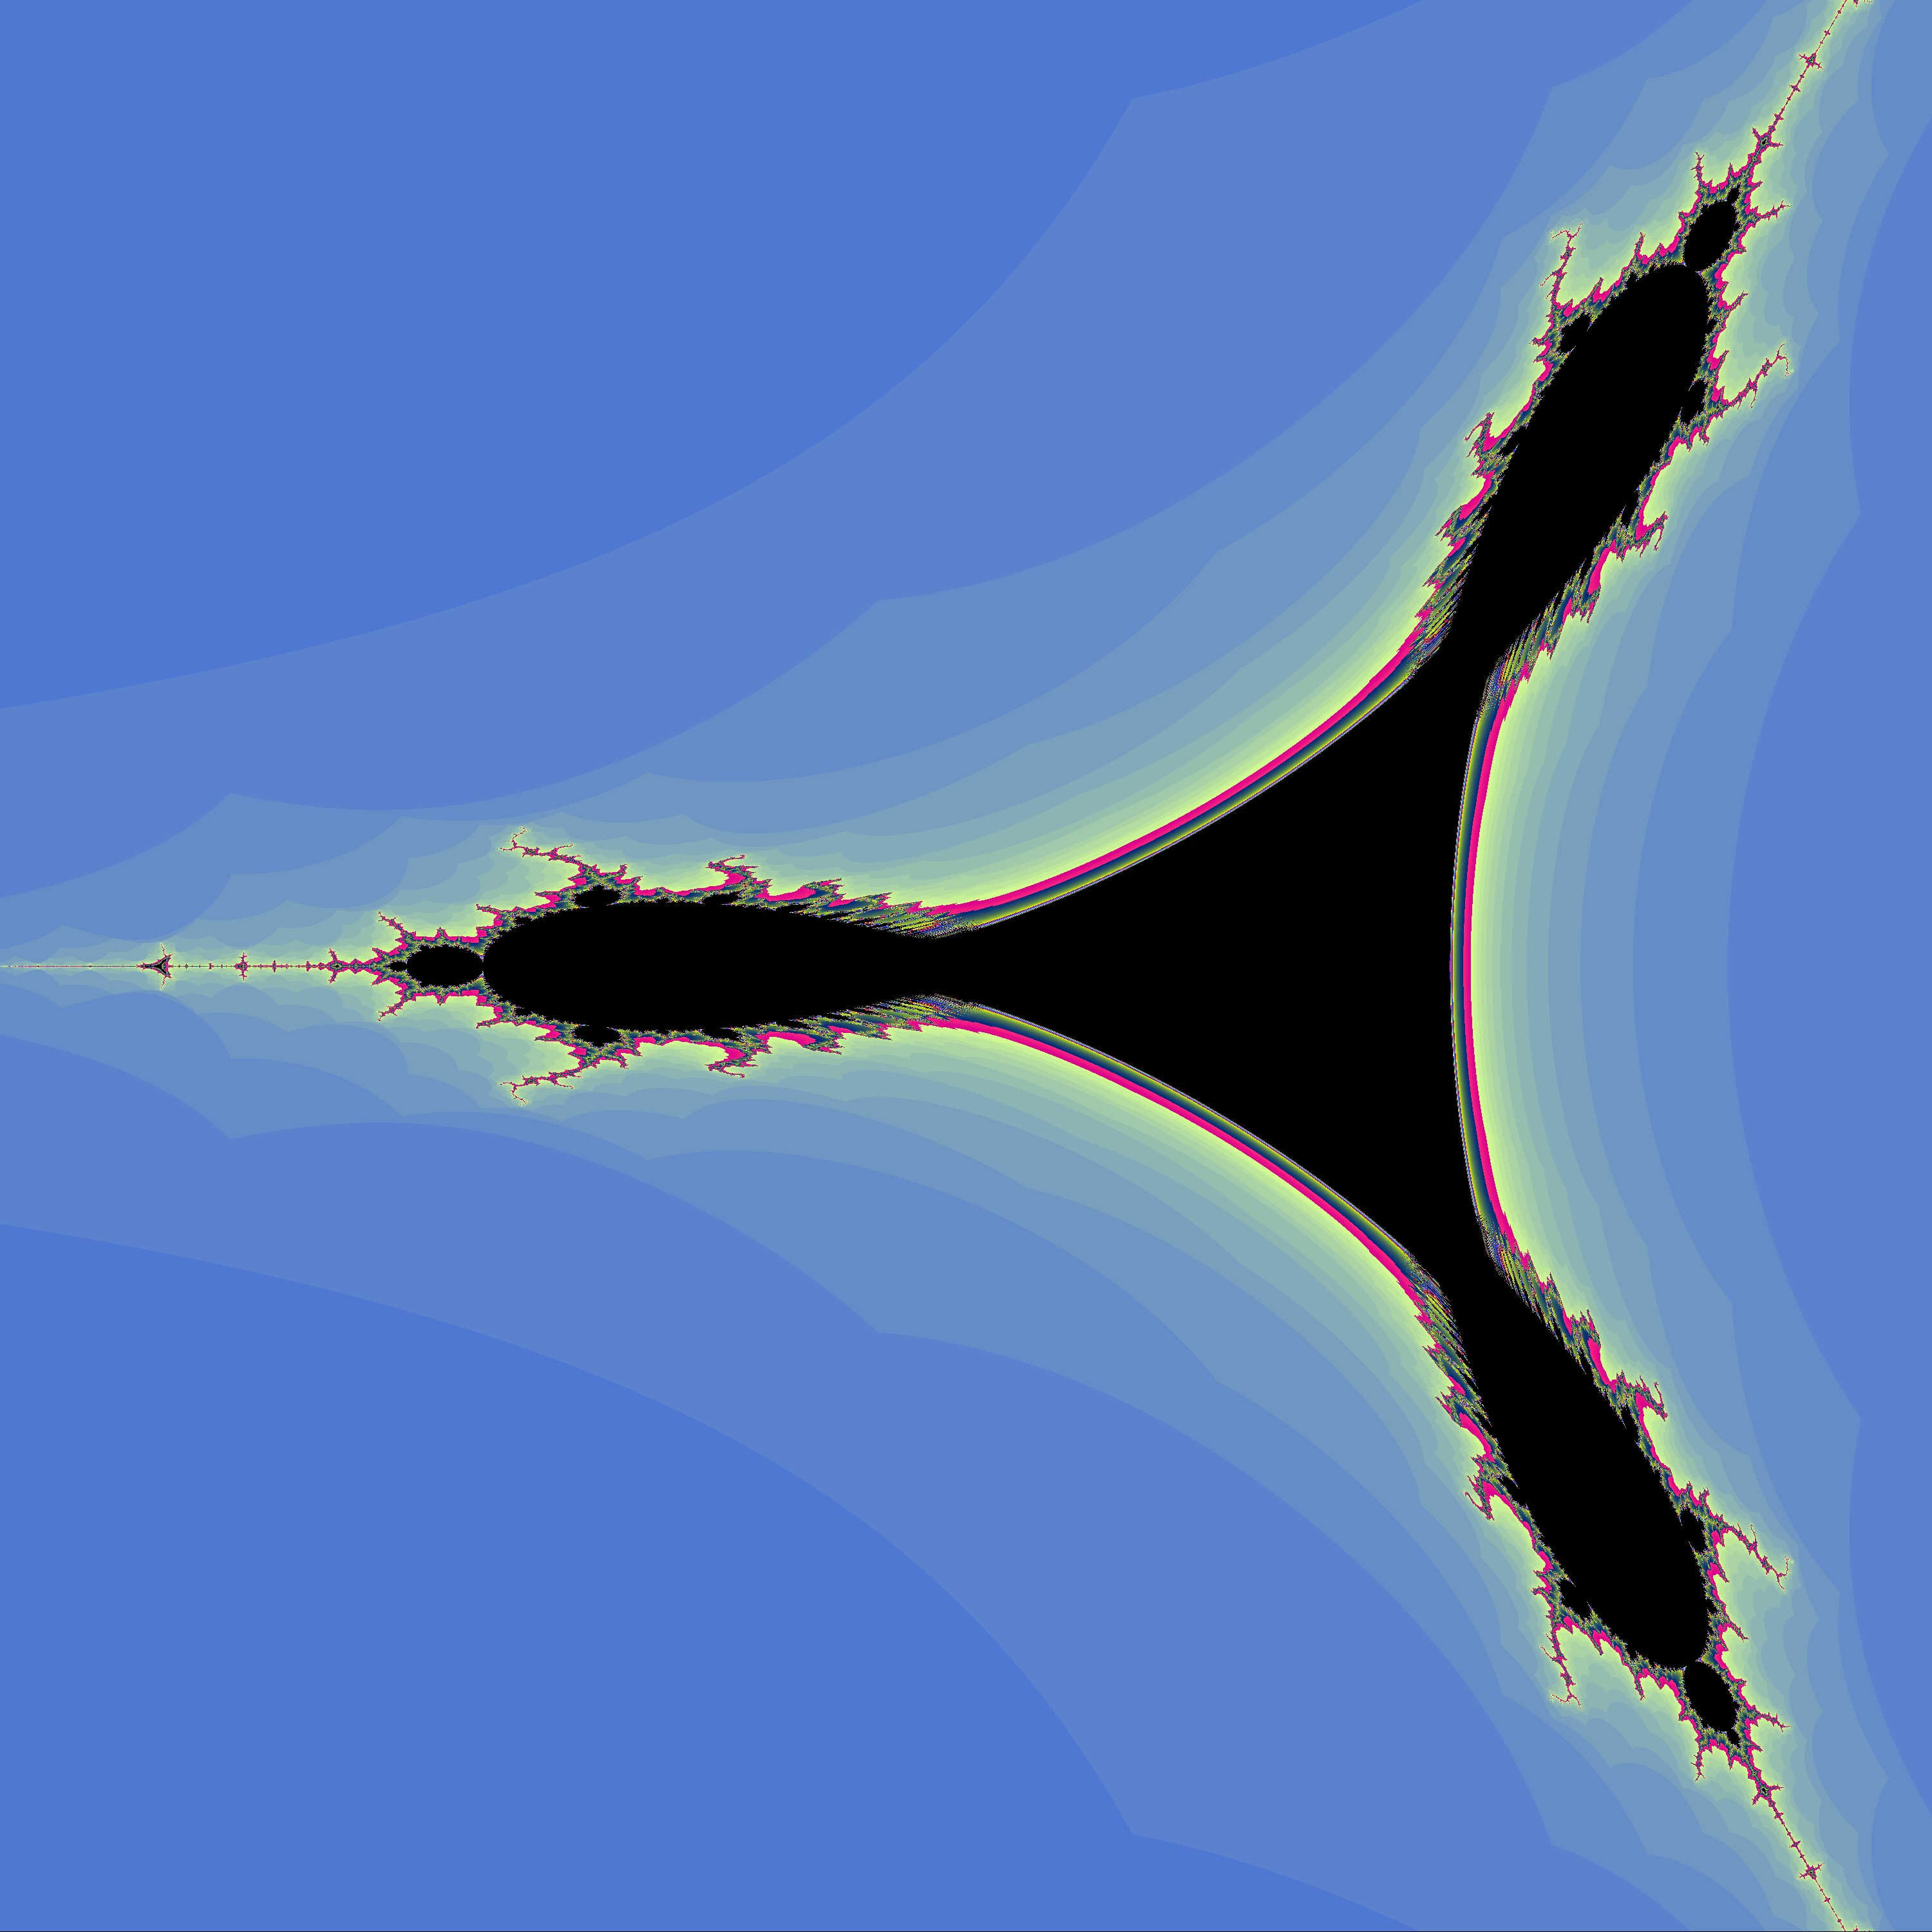
\includegraphics[width=60mm]{img/tricorn_result.jpg}
    \caption{Das Ergebnis unsere Implementierung nach ausf\"uhren von \lstinline{./main -2 -1 -1.5 1.5 1000}}
    \label{fig:tricorn_result}
\end{figure}

Man kann auch die durch \lstinline{make} generierte Dateien durch Ausf\"uhrung des Commandos \lstinline{make clean} schnell l\"oschen. 

\subsection{Entwickler Dokumentation}\label{sub:entwickler}

Unsere Implementierung haben wir mit C angefangen. Dann haben wir diese zu Assembler umgewandelt (wobei die ganzen I/O Operationen und die Konfiguration des Bitmaps in C blieben) und zuletzt haben wir die Parallelisierung mit Simd implementiert. In die n\"achsten Zeilen erkl\"aren wir die drei Implementierungen. 

\subsubsection{Erste Implementierung: C}

Da Assembler schwer f\"ur erste und schnelle Vorstellungen ist, haben wir unsere Ideen erstmal in C geschrieben. Wir hoffen dass, nach diese Erkl\"arung sich der Leser auch die grobe Funktionalit\"at des Programs versteht. \\

Hier haben wir die Funktionalit\"at in zwei Dateien unterteilt. Die Datei die sp\"ater in Assembler umgewandelt werden soll (\lstinline{tricorn.c}) und die Datei die nach die Erweiterung mit Assembler erhalten bleiben soll (\lstinline{main.c}), da dieser die I/O Operationen und die Konfiguration des Bitmaps macht.

\paragraph{main.c} 

\textbf{TODO: falta aqui explicar relativamente detalladamente, pues dar a entender que se hizo ahi, esto yo no lo puedo hacer muy bien, diria que Erick es el elegido}

\paragraph{tricorn.c}

In \lstinline{tricorn.c} berechnen wir die Formel des Tricorns (\ref{eq:tricorn}) f\"ur jedes $c$ innerhalb des eingesetzten Intervall und die eingesetzte Resolution. \\

Die erste Funktion ist \lstinline{void squareConjugate(float* result)}. Diese bekommt als Parameter einen zwei elementigen Array mit dem reellen (\lstinline{result[0]}) und imagin\"aren (\lstinline{result[1]}) Teil der einen gegebenen $z_i$ entsprechen soll. Diese Funktion wandelt also $z_i$ in $\overline{z_i}^2$. \\

Die zweite Funktion ist \lstinline{void complexAddition(float* result, float* c)}. Diese bekommt die komplexe Zahlen $z_i$ (\lstinline{result}) und $c$ (\lstinline{c}) als Parameter und f\"uhrt $z_i = z_i + c$ aus. \\

Danach kommt \lstinline{int check(float* z)} der 1 zur\"uckgibt wenn das gegebene z unstabil ist (d.h. wenn die Funktion aus dem Bereich $[-2, 2]$ f\"ur sowohl imagin\"are als auch reelle herausrutscht. Es gibt 0 aus wenn das gegebene $z_i$ (noch) unstabil ist. \\

Mit \lstinline{tricorn(float* z, float* c} wird durch ein gegebens aber fixes $z$ iteriert. Bei jede Iteration wird $\overline{z_i}^2$ berechnet und dann $c$ zu $z_i$ addiert. Dies geschieht bis der maximale Anzahl an Iterationen (wir haben uns ja davor f\"ur $R = 100$ entschieden) erreicht wird. Bei jede Iteration wird es geschaut, der Wert noch beschr\"ankt ist. Wenn dies nicht der Fall ist, wird der Anzahl an gebrauchte Iterationen zur\"uckgegeben. \\

Zuletzt, mit \lstinline{extern void multicorn_c(float r_start, float r_end, float i_start, float i_end, float res, unsigned char* img)} wird die Bildverarbeitung gemacht. Es wird erstmal die gesamte Anzahl an Bits berechnet, es wird das gen\"ugende Speicher alloziiert und dann wird es durch diesen Speicher (also das Bild) Reihe pro Reihe iteriert und unterschiedlich gemalt. Die Farbe wird von der Anzahl an Iterationen $i$ gemalt. 

\subsection{Assembler}

Nachdem wir mit unsere oben beschriebene Implementierung fertig geworden sind, haben wir \lstinline{tricorn.c} in Assembler umgewandelt. Dies geschah erstmal schrittweise, Funktion pro Funktion und am Ende sind zwei Dateien entstanden: \lstinline{tricorn.c} der, so wie oben, den Wert f\"ur einen $z_i$ berechnet. \\

Die gr\"o{\ss}te Ver\"anderung bez\"uglich C die durchgef\"uhrt wurde, liegt dem Arrays nahe: Wir benutzen den Speicher in Assembler nur f\"ur die Manipulation des Bildes. An sonsten haben wir uns entschieden, mehr Registern zu benutzen, da diese schneller sind. 

\textbf{TODO: terminar de explicar bien, si ha cambiado un poco el codigo desde lo que yo escribi, seria bueno si aqui alguien me apoya}

\subsection{Assembler SIMD}
\textbf{TODO:Hablar mas profundo de las funciones}

Für unsere Implementation der Parallelisierung haben wir uns entschieden gleichzeitig 4 Pixel zu berechnen. Nach jede Berechnungen von \lstinline{SquareConjugate_simd} und \lstinline{SquareAddition_simd} addieren wir ein Eins an der jeder Counter der Pixel der divergiert und ein Null an jeder der schon divergiert hat. Damit unsere Programm effizient funktioniert, gibt es ein ptest, der schaut ob alle unsere Incrementors Null sind und springt zur \lstinline{end_tricorn_simd}, weil in diesem Fall alle Pixel schon divergiert haben und ihre verschiedene Farben k\"onnen dargestellt werden.

\section{Ergebnisse}\label{section:ergebnisse}

\subsection{Benchmarking unsere Implementierungen}\label{sub:bench}

Die Tabelle \ref{tab:table1} \textbf{(Zeile = Implementierungen ; Spalte = Resolution)} zeigt wie sich unsere verschiedene Implementierungen von der Ausführungszeit \textbf{in Sekunden} unterscheiden. Erstmal die Implementierung die in C (mit -O3) geschrieben wurde, zeigt Zeiten die schneller als unsere synchrone Implementierung sind. Dies liegt an die Optimierung die gew\"ahlt wurde, denn diese \"ubersetzt das C Code in eine sehr optimale weise. Dies zeigt, dass unsere Implementierung in Assembler noch optimiert werden darf. \\

Die wichtigste Ergebnisse in der Tabelle werden in der letzte Zeile gezeigt. Diese zeigen, dass unsere paralelle Implementierung viel schneller ist, als sogar das Programm, der durch O3 optimiert wurde. Etwas wichtiges zu beachten ist, dass die Mehrheit der Pixel bei der Tricorn Fractal divergieren, und deswegen nur mit eine gro{\ss}e Resolution Variable wirklich den Unterschied sehen kann. 

\begin{table}[h!]\label{table:benchmarking}
  \begin{center}
    \label{tab:table1}
    \begin{tabular}{l|c|c|c|c|c|c}
      \textbf{} & \textbf{250} & \textbf{500} & \textbf{750} & \textbf{1000} & \textbf{2500} & \textbf{5000}\\ 
      \hline
        \rule{0pt}{25pt}\textbf{C} & 0.0454124 & 0.157775 & 0.3436602 & 0.605639 & 3.7216696 & 14.798096\\
        \hline
        \rule{0pt}{25pt}\textbf{ASM} & 0.0650032 & 0.2352244 & 0.5176214 & 0.9119462 & 5.649717 & 22.7363514\\
        \hline
        \rule{0pt}{25pt}\textbf{ASM\_SimD} & 0.03399 & 0.1066764 & 0.2285984 & 0.3981316 & 2.4923508 & 9.6546974\\

    \end{tabular}
    \caption{Prozessor Intel i5-5200U, Zeit für jede Implementierung in Sekunden. [Abb. \ref{fig:benchmark_result}]}
  \end{center}
\end{table}

\begin{figure}[ht]
    \centering
    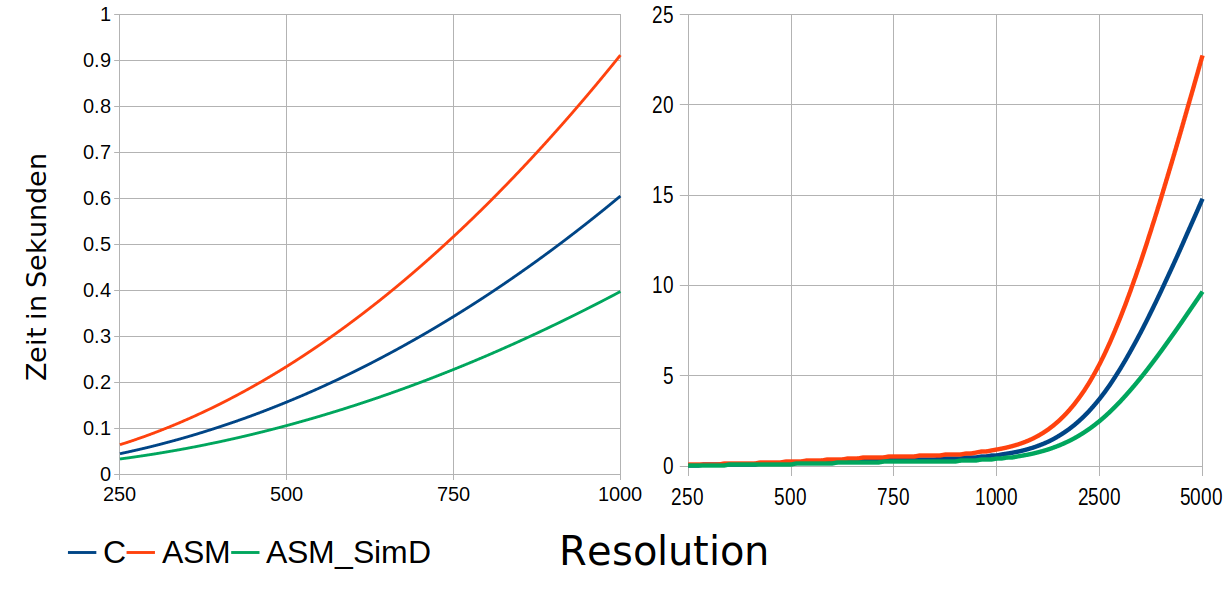
\includegraphics[width=140mm]{img/data_benchmarking.png}
    \caption{Wie verhalten sich die Daten von die Tabelle [\ref{tab:table1}]}
    \label{fig:benchmark_result}
\end{figure}

\section{Zusammenfassung}\label{section:zusammenfassung}

\textbf{TODO: resumen rapido, falta terminar el resto para hacerlo}

\subsection{Erweiterungsm\"oglichkeiten}

Wie durch einfaches betrachten des Bildes merkbar ist, kann man sehen, dass der reelle Axis eine Symetrieaxis bildet. Das hei{\ss}t, dass man die Berechnung einer sehr gro{\sse} Menge von Pixels gesparrt werden k\"onnte um somit die Berechnung noch schneller zu machen. Es ergibt sich also die Erweiterungsm\"oglichkeit einer graphischen Benutzeroberfläche, die die Eingabe eventuell noch einfacher gestaltet. Eine weitere naheliegende Idee ist, dem Programm auch die Berechnungen von andere Fraktals wie der Mandelbrot oder der Julia Set beizubringen.

\section{Quellenverzeichnis}\label{section:quellen}
\textbf{Yo quitaría Literatur y lo dejaría todo como Quellen de abajo}

\begin{thebibliography}{1}

\bibitem{tricorn_expected} 
 \href{https://en.wikipedia.org/wiki/Tricorn_(mathematics)#/media/File:Tricorn.png}{Wikipedia.org: A tricorn, created on a computer in C.}
 
 \bibitem{BMP_file_format} 
 \href{https://en.wikipedia.org/wiki/BMP_file_format)#/media/File:Tricorn.png}{Wikipedia.org: BMP File Format}

\end{thebibliography}

\end{document}
